\documentclass{book}
\usepackage[utf8]{inputenc}
\usepackage{indentfirst}	% make indent in first paragraph
\usepackage{bm}
\usepackage{geometry}		% to make typesettings like margins
\usepackage{mathrsfs}
\usepackage{amssymb}
\usepackage{hyperref}
\usepackage{amsmath}
\usepackage{natbib}			% to insert citations
\usepackage{xcolor}			% extend the colors can be used

\usepackage{bibentry}		% package used to insert full citation in body text
\nobibliography*

\usepackage{graphicx}		% to insert image
\graphicspath{ {images/} }

\usepackage[framemethod=default]{mdframed}
\usepackage{showexpl}
\mdfdefinestyle{comment}{
linecolor=gray,leftmargin=60,
rightmargin=40,
backgroundcolor=gray!10,
innertopmargin=4pt,
topline=false,leftline=false,bottomline=false,rightline=false}

\usepackage[english]{babel}
\renewcommand{\baselinestretch}{1.5}

\usepackage{amsthm}
\theoremstyle{plain}
\newtheorem{thm}{Theorem}[section] % reset theorem numbering for each chapter
\theoremstyle{definition}
\newtheorem{defn}[thm]{Definition} % definition numbers are dependent on theorem numbers
\newtheorem{exmp}[thm]{Example} % same for example numbers
\newtheorem{lemma}[thm]{Lemma}
\newtheorem{prop}{Proposition}
\newtheorem{obs}{Observation}

\citestyle{chicago}
\geometry{letterpaper, margin=1in}
% \setlength\parindent{0pt} % to cancel indent


% A list of new commands
\newcommand{\R}{\mathbb{R}}			% depends on the package amssymb



\title{Paper Notes}
\author{Kaida Zhang}
\date{}

\begin{document}

% \maketitle

\tableofcontents{}
\setcounter{tocdepth}{1}			% show only parts, chapters, and sections in content


\chapter{Econometrics}
\label{cha:econometrics}


\section{Low and Meghir, 2017, JEP} % (fold)
\label{sec:low_and_meghir_jep_2017}

\textbf{\bibentry{Low:2017jb}}\\

\textbf{Defining a structural model:}

A \textbf{fully specified model} make explicit assumptions about the economic actors' objectives and their economic enviroment and information set, as well as specifying which choices are being made within the model. They allow a complete solution to the individual's optimization problem as a function of current information set.
Fully specified models are particularly useful in understanding mechanism of a policy, especially when we want to estimate some long-term effects of the policy.

A \textbf{partially specified model} relies on a sufficient statistic that summarizes choices not being modeled specifically. For example, assuming that the choices is only intratemporal instead of intertemporal.

\textbf{Treatment effect models} focus on identifying a specific causal effect of a policy while saying least about the theoretical environment. The pro is the cleaness of causality. The con is the limitation in exploiting the results outside. The identification of treatment model depends on assumptions that the experienment has not been compromised and there is no spillovers from the treatment units.

A combination of fully speficied model and randomized experiments can enhance anaysis for both. Experimental evidence can be used either to validate a structural model, or to aid in the estimation process (in identification).

\textbf{Solving structural models}

This has been described in Adda and Cooper(2003) well. 
The general process is: 
1) write down the bellmand function;
2) discrete the state space and decision space;
3) use value function iteration to solve the bellman function.


% section low_and_meghir_jep_2017 (end)


\section{Lewbel, 2016, JEL} % (fold)
\label{sec:lewbel_2016_jel}

\textbf{\bibentry{Lewbel:2016wn}}\\

\url{https://www2.bc.edu/arthur-lewbel/ident-zoo-SL-Part1.pdf} 

\url{https://www2.bc.edu/arthur-lewbel/ident-zoo-SL-Part2.pdf}

are links for a ppt on this paper by Lewbel.\\

There are two kinds of identification problems. 
1. One is to identify the treatment effect, a typical example is the selection bias. The problem in these cases are that selection (determing who is treated or observed) and outcomes may be correlated. 
2. Another is to identify the true coefficient in a linear regression when regressors are measureed with error.

\subsection{Point Identification} % (fold)
\label{sub:point_identification}

We start by assuming some information $\phi$ is knowable. A simple definition of point identification is that a parameter $\theta$ is point identified if, given the model, is uniquely determined from $\phi$. Notice that this definition of point identification is recursive in some sense. To identify $\theta$, we first need to assume some $\phi$ is knowable, which means $\phi$ itself is identified. This identification of $\phi$ can only be justified by further assumptions of DGP (Data Generating Process).

For example, for a model $Y = X\theta +e$, we assume that $E(E^2)\ne0$ and $E(eX)=0$, and suppose $\phi$ includes the second order of $(Y,X)$. Then we can conclude that $\phi$ is point identified, given by $E(XY)/E(X^2)$. Notice that the identification comes from the \textit{assumptions} of model.

One common DGP is IID. Under this DGP, we can consistently indentify the distribution of observation W. Another DGP is where each data point consists of a value of X chosen from its support, then we randomly draw Y conditional on X, which is independent from other draws conditional on this X. Under this DGP, we can consistently identify $F(Y|X)$. We can also use more complicated DGPs, for example, we generally assume only the second order moments are knowable in time series. One reason is this being sufficient for identification, another reason is higher order moments become unstable over time. Assumptions over GDP are always needed, even in experienment data, and which specific assumptions to take depend on the model.


% subsection point_identification (end)

% section lewbel_2016_jel (end)


% chapter econometrics (end)



%%%%%%%%%%%%%%%%%%%%%%%%%%%%%%%%% IO %%%%%%%%%%%%%%%%%%%%%%

\chapter{IO} % (fold)
\label{cha:io}

\section{Rey and Stiglitz, 1995, RAND} % (fold)
\label{sec:rey_and_stiglitz_1995_rand}

\textbf{\bibentry{Rey:1995ft}}

For detailed proof of this paper, see Evernote.\\

\textbf{Main result:}
vertical restrains can be used to reduce interband competition. Because exclusive territories alter the perceived demand curve, making each producer believe he faces a less elastic demand curve, inducing an increase in eqm price and producer's profits even in the abscence of franchise fee. This result is different from traditional Chicago school results, which insist that exclusive terittories will increase efficiency. This difference comes from market structure. Chicago schools investigate in full competition and full monopoly producer cases, while this paper looks at duopoly producer. In full competition and full monopoly case, the competition level has already been \textit{preassumed}, while exclusive territories can reduce the competition level among producers in other cases.\\

The key for the result is the the following compound demand elastic:
\[\tilde\varepsilon(p^e):=m_1(p,p)\varepsilon_1(q,q)+m_2(p,p)\varepsilon_2(q,q) \]
where $q=q_1^r(p,p)$ (the response retail price),
$m_1(p,p)=\partial \log q_1^r(p_1,p_2)/\partial \log p_1$ (the own elasticity of retail price to producer price),
and  $m_2(p,p)=\partial \log q_1^r(p_1,p_2)/\partial \log p_2$ (the cross elasticity of retail price to producer price),
and $\varepsilon_1(q_1,q_2)=-\partial \log D^1(q_1,q_2)/q_1$ (the own elasticity of demand to retail price, positive),
and $\varepsilon_2(q_1,q_2)=-\partial \log D^1(q_1,q_2)/q_2$ (the cross elasticity of demand to retail price, negative).

In the above equation, it is very reasonable to think $0<m_1<1$ and $0<m_2$. $m_1>0$ because the own elasticity of retail price to producer price is positive. $m_1<1$ means that retailer will absorb some increase in producers' price, which will be the case if demand elasticity becomes higher in high retail price. And $0<m_2$ derives from the two products to be substitutes. Under these two conditions, combined with $\varepsilon_1>0$ and $\varepsilon_2<0$, then $\tilde\varepsilon(p^e)<\varepsilon_1$. Thus, under exclusive territories, the producers' perceived demand curve is less elastic. So the equilibrium price (both retail and producer) is higher even when no franchise fee applies.

\noindent
\textbf{Setting:}

\begin{itemize}
	\item two manufacturers produce imperfect substitutes at same marginal cost \textit{c}
	\item retailers are perfect competition / or exclusive territory
	\item the final good demand depends on retail prices and is given by $D^i(q_1,q_2)$
	\item costs and demand functions are common knowledge, retailers observe all contracts signed by each producer
	\item producers only observer the quantity bought by retailers; they do not observe the quantities sold by retailers (i.e. fullline forcing is infeasible)
	\item producers serve many markets at no addtional cost
	\item consumers have no search cost
\end{itemize}

Under these settings and information conditions, we can see it as a two stave game. In the first stage, producers simultaneously set wholesale price $p_1$ and $p_2$. In the second stage, the retailer observe all wholesale price and decide the retail price simutaneously.

\subsection{Benchmark Case} % (fold)
\label{sub:benchmark}

We use the following assumptions throughout the paper unless specified otherwise:

\begin{enumerate}
	\item Let $\pi(p_i,q_1,q_2) := (q_i-p_i)D^i(q_1,q_2)$ denote the retail profit for product i; assume it to be twice differentiable wrt each argument, and is sigle peaked wrt $q_i$. The reaction function $q_i^a(p_i,q_j)$ is thus continously differentiable and characterized by FOC.
	\item Products are substitutes: $\partial D^i/\partial q_i \leq 0$ and $\partial D^i/\partial q_j \geq 0$
	\item Demand functions are symmetric: $\forall p_1,p_2 \in \R_+, D^1(p_1,p_2) = D^2(p_2,p_1)$
\end{enumerate}

Think of the benckmark case that no vertical restriction so the retailers are perfect competitive, and the producer monopolizes. In this case, the game is just a one step optimal pricing problem. The producer chooses an optimal retail price.\\

\begin{mdframed}[style=comment]

\noindent
\textbf{Useful trick:}

Throughout this paper, we can write the symmetric eqm conditions in the following form:
\[(p^c - c)/p^c=1/\varepsilon(p^c,p^c)\]
where $p^c$ is the symmetric eqm price, and $\varepsilon$ is some kind of elasticity.

In a symmetric eqm, the FOC of each producer gives 
\((p^c - c)/p^c=1/\varepsilon_1(p^c,p^c)\)
where $\varepsilon_1 = -\partial \log D^1(q_1,q_2)/\partial \log q_1$, i.e. the self elasticity of demand.

In the simplest benchmark case, the two factories are integrated, leading us to:
\((p^c - c)/p^c=1/E(q^m)\),
$E(q):=\varepsilon_1(q,q)+\varepsilon_2(q,q)$, where $\varepsilon_2 = -\partial \log D^1(q_1,q_2)/\partial \log q_2$ (the cross demand elasticity).

In the exclusive territory case, the symmetric eqm satisfies \((p^e - c)/p^e=1/\tilde\varepsilon(p^e)\), where 
\[\tilde\varepsilon(p^e):=m_1(p,p)\varepsilon_1(q,q)+m_2(p,p)\varepsilon_2(q,q) \]
where $q=q_1^r(p,p)$ (the response retail price),
$m_1(p,p)=\partial \log q_1^r(p_1,p_2)/\partial \log p_1$ (the own elasticity of retail price to producer price),
and  $m_2(p,p)=\partial \log q_1^r(p_1,p_2)/\partial \log p_2$ (the cross elasticity of retail price to producer price).

\end{mdframed}




% subsection benchmark (end)


% section patrick_and_stiglitz_1995_rand (end)

\section{Production Function Estimation} % (fold)
\label{sec:production_function_estimation}

There are several difficulties in estimating production functions which will cause endogeneity problem. To name some:
\begin{itemize}
	\item Simultaneouty. For a production function like $y_{it}=\beta_0+\beta_1 k_{it}+\beta_2 l_{it} + \omega_{it}+\varepsilon_{it}$, we suppose that $\omega_{it}$ is obseved by firm but not by econometricians, and $\varepsilon_{it}$ is observed neither by firm nor econometrician. This could induce endogeneity when directly using OLS. Suppose $\omega_{it}$ has positive serial correlation, when $\omega_{it}$ is high, firm will choose higher input bacause it is very possible that $\omega$ in next period will be high as well. This induces a positive bias for $\beta_k$.
	\item Exit selection bias. When constructing a balanced panel, then we only observe those firms with high $\omega_{it}$.
\end{itemize}

There are several approaches in solving this problem.

\begin{itemize}
	\item Classical Approach.
	\begin{itemize}
		\item Use input price as IV. The problem is input price is generally the same across firms. When we do observe different input prices, which generally indicates market power in input markets. Thus those facing higher $\omega_i$ will tend to produce more, inducing their input price to increase, which has a negative bias on $\beta_k$.
		\item Use fixed effect. We need to assume that a firm faces same $\omega_{it}$ across time, which is not very practical.
	\end{itemize}
	\item Control Function for  $\omega_{it}$. This approach first raised by \cite{Olley:1996ef} and developed by \cite{Levinsohn:2003ej} and \cite{Ackerberg:2015ha}. We name them OP, LP, ACF here after. The key idea is to use a function of what we know (for example, $k_t$ and $i_{t-1}$ in OP) to proxy $\omega$, the existence of such function is guaranteed by the solutioin property of the firm optimization problem. And the specific form of this function is estimated nonparametrically.
	\begin{itemize}
		\item OP uses a two step estimation process. First step, use $k_t$ and $i_{t-1}$ nonparametrically estimate $\omega_t$, plug this into original production function then use OLS. Notice the unobserved $\omega_t$ has been controled by $k_t$ and $i_{t-1}$, then OLS will give consistent estimator for $l_t$ but not $k_t$. In second step, we first write $\omega_{it} = E[\omega_{it}|\omega_{it-1}]+\xi_{it}$, notice that $\xi_{it}$ is independent of any information set at t-1. Thus we get the moment condition $E[\xi_{it}k_{it}]=0$, then we can use method of simulating moments to estimate $\beta_k$.
		\item LP is very similar to OP, just that use intermediate input $m_{it}$ instead of investment $i_{it}$ in proxy $\omega_{it}$. Because OP approach requires the policy function of $i_{it}$ be monotonicity in $\omega_{it}$, which is unsatisfied when $i_{it}=0$. But data shows that in many observations $i=0$. Using intermediate input can solve this.
		\item ACF critizition is
	\end{itemize}
	\item \cite{Gandhi:2017un} Approach (GNR). GNR criticizes control function approach is nonparametrically not identified in the presence of flexible inputs. They raise a new approach using FOC conditions.
\end{itemize}


% section production_function_estimation (end)





% chapter io (end)



\chapter{Decision Theory} % (fold)
\label{cha:decision_theory}

\section{Dekel and Lipman, 2010, Annu Rev Econ} % (fold)
\label{sec:dekel_and_lipman_2010_annu_rev_econ}

\textbf{\bibentry{Dekel:2010bm}}\\

\noindent
\textbf{What we can learn from decision theory}

1) to know whether our intuition is correct;
2) to flesh out initial intuition to get additional or better prediction (e.g. some additional observable prediction);
3) to help us understand of why and how mechanism works

\noindent
\textbf{Story of the model}

Why the story of the model is important even if it is not realistic? Why we can't just choose the model by the 'prediction-rejection' procedure?

1) The story makes us believe the predictions more;
2) Having a nice intuition helps us to utilize the model and to expand the model;
3) And a model can never be realistic, the important thing is whether it captures something important.


% section dekel_and_lipman_2010_annu_rev_econ (end)

% chapter decision_theory (end)

\chapter{Matching Theory} % (fold)
\label{cha:matching_theory}

\section{Gale and Shapley, 1962, Ame.Math.Mon.} % (fold)
\label{sec:gale_and_shapley_1962}

\textbf{\bibentry{Gale:1962kl}}

This paper introduces Deffered Acceptance (DA) algorithms in matching, and shows that it is stable and optimal.

\begin{defn}
An assignment is called \textbf{unstable} if there are two applicants $\alpha$ and $\beta$ who are assigned to universities A and B, although $\beta$ prefers A to B and A prefers $\beta$ to $\alpha$.
\end{defn}

\begin{defn}
A stable assignment is called \textbf{optimal} if \textit{every} applicant is at least as well off under it as under any other stable assignments.
\end{defn}

Comment: it loos at first that optimal assignments may not always exist. But as we will show constructively, it does.

\begin{defn}
\textbf{Deferred Acceptance algorithm} works as following. First let each boy propose to his favorite girl. Each girl who receives more than one proposal rejects all but her favorite boy. Yet, she doesn't accept him, but keeps him in a string to allow for the better may come later. Then in the second round, each rejected boy propose their second favorite girl, and each girl picks her favorite among the new proposers and the one in the string, and put him in her string. This process continues, until each girl has one boy in the string (this will happen after finite rounds), then each girl picks the boy in her string.
\end{defn}

We will show the assignment by above algorithm is stable and optimal.

% section gale_and_shapley_1962 (end)


% chapter matching_theory (end)






\chapter{Macro} % (fold)
\label{cha:chapter_name}

\section{Kiyotaki, 2011} % (fold)
\label{sec:kiyotaki_2011}

\textbf{\bibentry{Kiyotaki:2011fc}}

This paper mainly discusses the micro structures which may induce financial friction (inefficiency). These structures include private information of income, private technology for storage, limited commitment and their combinations.



% section kiyotaki_2011 (end)


\section{Costly State Verification} % (fold)
\label{sec:costly_state_verification}

Financial frictions is an important yet not well explained phenomena. Generally financial frictions means some possible financial frictions not happening, resulting in fluctuations in real economy. There are several micro foundations for financial frictions, we learned some in Ruilin's course:
\begin{itemize}
	\item costly state verification
	\item collateral constraints
	\item moral hazard
	\item asymmetric information
\end{itemize}

The main framework for costly state verification is following. The borrower has some private information on productivity, and lender has to pay some cost to get this information. This will give the borrower some advantage, and make some possible transactions unable to happen. \cite{Townsend:1979ef} gives a micro model describing contract under costly state verification. \cite{BenBernanke:1989eg} and \cite{Carlstrom:1997fb} are two important works using this to explain business cycles (also called Financial Accelarator).

\textcolor{red}{Add breif introduction for costly state verification literature.}


% section costly_state_verification (end)

\section{Collateral Constraints} % (fold)
\label{sec:collateral_constraints}


Another explaination for financial friction is collateral constraint. Important literatures include \cite{Kiyotaki:1997hl},

\cite{Kiyotaki:1997hl} has a simple idea. Suppose the borrower needs some collateral (say land) for borrowing. What is the effect of a temporary increase in land productivity? The direct effect is it will increase this period land price. More important is the indirect effect, the borrower now can buy more land since their collateral becomes more valuable. And thus in next period they can buy even more land. This long chain has a large effect on the initial price of the land. Thus financial sector can amplify the fluctuation of real economy.

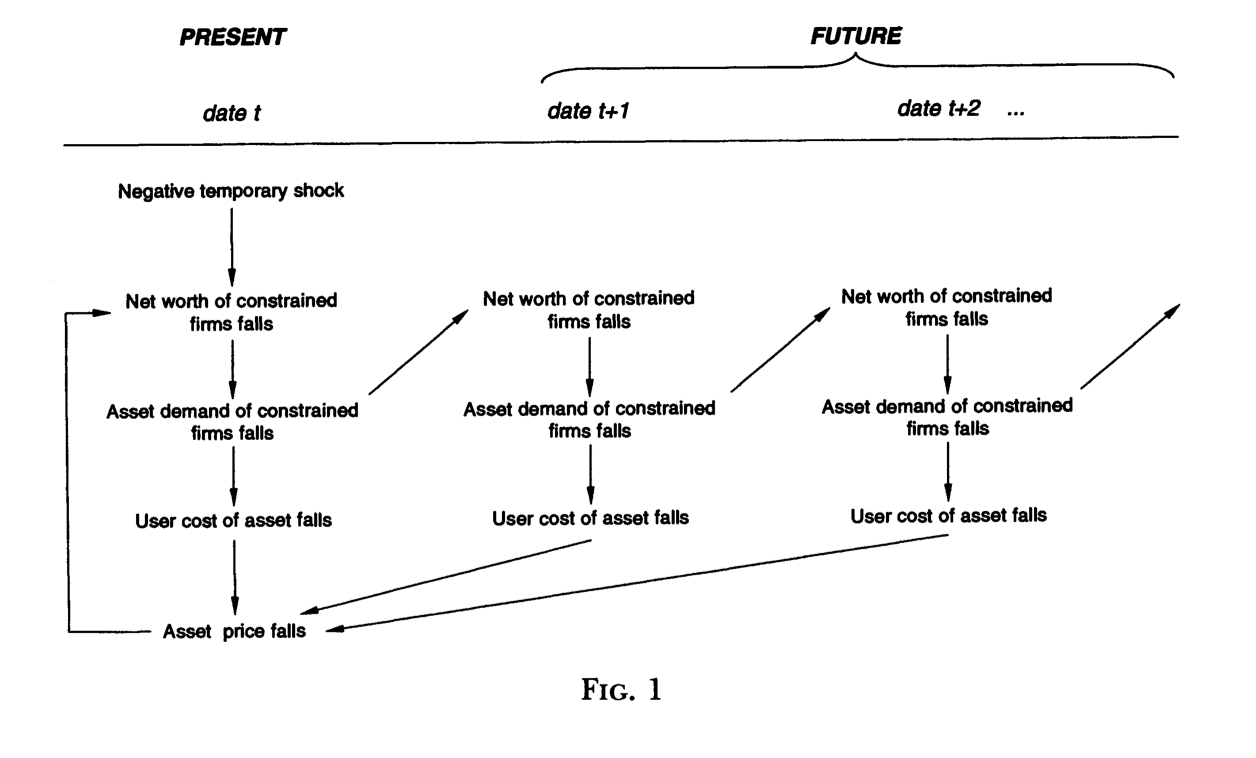
\includegraphics[width=\textwidth]{kiyotaki-moore-97.png}


% section collateral_constraints (end)



% chapter macro (end)


\chapter{General (mathematical) Skills} % (fold)
\label{cha:general_mathematical_skills}

\section{Log-Linearization}

\noindent
\textbf{Motivation}

Why we need log linearizations?
Because for most nonlinear discrete dynamic programming problems,
we fail to find a closed solution.
Thus we have to use numerical method or to find a approximation.
By using log-linearization,
we transform the nonlinear problem to a linear problem (around the steady state),
and we know how to solve the linear diffrence equations.

Another advantege of log-linearization is,
the new variables are in forms of $\frac{x-x^*}{x^*}$,
which is interpretable.\\


% subsection: how to do log-linearization
\subsection{How to do Log-Linearization}

Log linearization is a common method to approximate non-linear function using Taylor expansion.

When we do linearization in macroeconomics, one key is to find \emph{\textbf{steady state}} of the model.
Then we do linearization aroud the steady state.

The basic idea is, for functions like:
\[f(x)=\frac{g(x)}{h(x)}\]

take log in both sides:
\[ln(f(x))=ln(g(x))-ln(h(x))\]

By Taylor expansion, for a smooth function f(x) we have:
\[f(x)=f(x^*)+\frac{f'(x^*)}{1!}(x-x^*)+o(1)\]

Thus 
\[lnf(x) \approx lnf(x^*)+\frac{f'(x^*)}{f(x^*)}(x-x^*)\]

The above follows from the fact that $\frac{dln(f(x))}{dx}=\frac{f'(x)}{f(x)}$. Thus,
\[lnf(x)-lnf(x^*)=\frac{f'(x^*)}{f(x^*)} \cdot x^* \cdot \frac{x-x^*}{x^*}\]

And the equation becomes:
\[lnf(x^*)+\frac{f'(x^*)}{f(x^*)} \cdot x^* \cdot \frac{x-x^*}{x^*}=lng(x^*)-lnh(x^*)
\frac{g'(x^*)}{g(x^*)} \cdot x^* \cdot \frac{x-x^*}{x^*}-
\frac{h'(x^*)}{h(x^*)} \cdot x^* \cdot \frac{x-x^*}{x^*}\]

\[\frac{f'(x^*)}{f(x^*)} \cdot x^* \cdot \frac{x-x^*}{x^*}=
\frac{g'(x^*)}{g(x^*)} \cdot x^* \cdot \frac{x-x^*}{x^*}-
\frac{h'(x^*)}{h(x^*)} \cdot x^* \cdot \frac{x-x^*}{x^*}\]

Dedine $\hat x=\frac{x-x^*}{x^*}$, and we are done.
\[\frac{f'(x^*)}{f(x^*)} x^* \cdot \hat x=
\frac{g'(x^*)}{g(x^*)} x^* \cdot \hat x-
\frac{h'(x^*)}{h(x^*)} x^* \cdot \hat x\]

Notice, when we use $\hat x$ in place of $x-x^*$in the approximation,
don't forget to times $x^*$ !!\\

% How to do log-linearization when there is Expectation

\subsection{log-linearization when there is expectation (An Example)}

It may be annoying to do log-linearization when there is expectation,
because in general,
log and expectation cannot switch.
But if we don't switch, we cannot do the log-linearization as previous.
For example, see Adda\&Cooper(2003) CH5, page 115.

Suppose we have the following Euler equation:

\[u'(c)=\beta E_{A'|A}u'(c)[Af'(k')+(1-\delta)]\]

where $c=Af(k)+(1-\delta)k-k'$.

These two expressions, along with the evolution of A,
defines a system of equations.

In this system, actually we do not have to take log,
but directly do Taylor expansion at $c^*$, $x^*$ and $k^*$.
We get:

\begin{multline}
u'(c^*)+u''(c^*)c^*\hat c_t=
\beta E_{A'|A}[u'(c^*)(\bar Af'(k^*)+(1-\delta))
+(\bar Af'(k^*)+(1-\delta))u''(c^*)c^*\hat c_{t+1}\\
+u'(c^*)f'(k^*)\bar A\hat A_{t+1}+
u'(c^*)\bar Af''(k^*)k^* \hat k_{t+1}]
\end{multline}


The first term in LHS and the first term in RHS cancel each other.
And we divide both sides by $u'(c^*)$, and we will get:

\begin{equation}\label{eq1}
\frac{u''(c^*)c^*}{u'(c^*)}\hat c_t
=\beta E_{A|A'}[\frac{u''(c^*)c^*}{u'(c^*)}\hat c_{t+1} \frac{1}{\beta}
+f'(k^*)\bar A \hat A{t+1}
+f''(k^*)k^*\hat k_{t+1}]
\end{equation}

Notice, we derive this based on the fact $\frac{1}{\beta}=\bar A f'(k^*)+(1-\delta)$.
Because by FOC
\[u'(c)=\beta E_{A'|A}V'(k')\]

To derive $V'(k')$, we first derive $V'(k)$,
by Envelop THM we get:
\[V'(k)=u'(c)[Af'(k)+(1-\delta)]\]

Substitute this into FOC we get:
\[u'(c)=\beta E_{A|A'}[u'(c')(A'f'(k')+(1-\delta))]\]

In this approach we fix A at the mean $\bar A$,
and thus the steady state satisfy:
\[1=\beta [\bar Af'(k^*)+(1-\delta)]\]

Here, the introduce of $\bar A$ is to describe the steady state in existence of shock.
We can see $\bar A$ as the "long term" growth of the economy,
and the we investigate what's the optimal steady $k^*$ under this long-term growth rate.

\textcolor{red}
{But I still don't know why we can cancel the expectation in the RHS.}

The equation \ref{eq1} is the linear function we want.\\

\noindent
\emph{Some Comments on the above method:}

Although it seems that the above method uses no log-linearization,
actually it does!

(to be added later)

% section log-linearization (end)

% chapter general_mathematical_skills (end)



\renewcommand\refname{Reference}
\bibliographystyle{plainnat}
\bibliography{paper_notes}


\end{document}
